\documentclass[journal=jacsat,manuscript=article]{achemso}

\usepackage{hyperref}
\usepackage{graphicx}
\usepackage{array}

\graphicspath{ {./resources/} }
\newcolumntype{P}[1]{>{\centering\arraybackslash}p{#1}}


%%%%%%%%%%%%%%%%%%%%%%%%%%%%%%%%%%%%%%%%%%%%%%%%%%%%%%%%%%%%%%%%%%%%%
%% If issues arise when submitting your manuscript, you may want to
%% un-comment the next line.  This provides information on the
%% version of every file you have used.
%%%%%%%%%%%%%%%%%%%%%%%%%%%%%%%%%%%%%%%%%%%%%%%%%%%%%%%%%%%%%%%%%%%%%
% \listfiles

\newcommand*\mycommand[1]{\texttt{\emph{#1}}}
\renewcommand{\thefootnote}{\fnsymbol{footnote}}

\author{Vineeth R. Chelur}
\author{U. Deva Priyakumar}
\email{deva@iiit.ac.in}
% \phone{+91 9490441430}
\affiliation[IIIT-H]
{Center for Computational Natural Sciences \& Bioinformatics \\ International Institute of Information Technology \\ Hyderabad - 500032, India}

\title[BiRDS - Binding Residue Detection from Protein Sequences using Deep ResNets]
  {BiRDS - Binding Residue Detection from Protein Sequences using Deep ResNets
%   \footnote{A footnote for the title}
  }

%%%%%%%%%%%%%%%%%%%%%%%%%%%%%%%%%%%%%%%%%%%%%%%%%%%%%%%%%%%%%%%%%%%%%
%% Some journals require a list of abbreviations or keywords to be
%% supplied. These should be set up here and will be printed after
%% the title and author information, if needed.
%%%%%%%%%%%%%%%%%%%%%%%%%%%%%%%%%%%%%%%%%%%%%%%%%%%%%%%%%%%%%%%%%%%%%
% \abbreviations{IR,NMR,UV}
% \keywords{American Chemical Society, \LaTeX}

\begin{document}

%%%%%%%%%%%%%%%%%%%%%%%%%%%%%%%%%%%%%%%%%%%%%%%%%%%%%%%%%%%%%%%%%%%%%
%% The "tocentry" environment can be used to create an entry for the
%% graphical table of contents. It is given here as some journals
%% require that it is printed as part of the abstract page. It will
%% be automatically moved as appropriate.
%%%%%%%%%%%%%%%%%%%%%%%%%%%%%%%%%%%%%%%%%%%%%%%%%%%%%%%%%%%%%%%%%%%%%
% \begin{tocentry}

% Some journals require a graphical entry for the Table of Contents.
% This should be laid out ``print ready'' so that the sizing of the
% text is correct.

% Inside the \texttt{tocentry} environment, the font used is Helvetica
% 8\,pt, as required by \emph{Journal of the American Chemical
% Society}.

% The surrounding frame is 9\,cm by 3.5\,cm, which is the maximum
% permitted for  \emph{Journal of the American Chemical Society}
% graphical table of content entries. The box will not resize if the
% content is too big: instead it will overflow the edge of the box.

% This box and the associated title will always be printed on a
% separate page at the end of the document.

% \end{tocentry}

\begin{abstract}
    \noindent Protein-drug interactions play important roles in many biological processes and therapeutics. Prediction of the active binding site of a protein helps discover and optimise these interactions leading to the design of better ligand molecules. The tertiary structure of a protein determines the binding sites available to the drug molecule. However, the methods for structure determination are labour-intensive and time-consuming. A quick and accurate prediction of the binding site from sequence alone would help speed up drug design when the structure becomes available. Deep Learning has been used in a variety of biochemical tasks and has been hugely successful. In this paper, a Residual Neural Network (leveraging skip connections) is implemented to predict a protein's most active binding site. An Annotated Database of Druggable Binding Sites from the Protein DataBank, sc-PDB, is used for training the network. Features extracted from the Multiple Sequence Alignments (MSAs) of the protein generated using DeepMSA, such as Position-Specific Scoring Matrix (PSSM), Secondary Structure (SS3), and Relative Solvent Accessibility (RSA), are provided as input to the network. A weighted binary cross-entropy loss function is used to counter the substantial imbalance in the two classes of binding and non-binding residues. The network performs very well on single-chain proteins, providing a pocket that has good interactions with a ligand.
\end{abstract}

\section{Introduction}
\quad The rapid speed of sequencing attained with modern DNA sequencing technology has been instrumental in sequencing complete DNA sequences, which leads to faster sequencing of proteins. Although there have been improvements in the determination of the three-dimensional protein structure by techniques such as X-ray Crystallography, NMR Spectroscopy and Cryo-Electron Microscopy, the gap between the number of known protein sequences (214,406,399 UniProt sequences as of May 2021)\cite{uniprot2021uniprot}, and the number of known structures (177,910 PDBs as of May 2021)\cite{berman2000protein}\cite{burley2021rcsb} is large. Proteins perform a vast array of functions within organisms, and the tertiary structure of a protein can provide important clues about these functions.

In drug design, new drugs are designed based on the knowledge of a biological target such as a protein. The identification of the potential active binding site of a protein is an essential step in drug design. Predicting the binding site of a protein, based on sequence alone, helps speed up the process of drug design by having a binding site ready for testing when the structure becomes available. Ligand binding site prediction methods can be clustered into four groups: 3D structure-based, template similarity-based, traditional machine learning-based and deep learning-based prediction methods.

Three-dimensional structure-based methods assume that most small ligand bindings occur in cavities on protein surfaces because large interfaces have a high affinity. Hence, these methods locate the binding site by searching for spatial geometry or energy features (by placing probes) in protein structures. SITEHOUND \cite{hernandez2009sitehound} uses a carbon and phosphate probe inside a grid that covers the entire protein. The grid points with higher interaction energies are clustered and determine the binding residues. CURPOCKET \cite{liu2020cb} is a spatial geometric measurement method that computes the curvature distribution of the protein surface and identifies clusters of concave regions. Some other methods include CASTp \cite{dundas2006castp}, LIGSITE \cite{hendlich1997ligsite}, VISCANA \cite{amari2006viscana}, Fpocket \cite{le2009fpocket}, Patch-Surfer2.0 \cite{zhu2015large}. While 3D structure-based methods have been widely used, they depend on various factors such as the resolution of the structure determination method, the presence or absence of ligand groups, and external molecules.

Template similarity-based methods do not consider proteins as independent entities but evolved from structurally, functionally or sequentially similar proteins. S-SITE and TM-SITE \cite{yang2013protein} employ the Needleman-Wunsch algorithm to align the query protein to each of the proteins in the BioLip \cite{yang2012biolip} database and selects similar sequences according to the alignment. The binding residues of the aligned proteins, which occur more frequently, are considered the binding site. Methods such as ConSurf \cite{glaser2003consurf}, FINDSITE \cite{brylinski2008threading}, 3DLigandSite \cite{wass20103dligandsite}, FunFOLD \cite{roche2011funfold}, COFACTOR \cite{roy2012recognizing}, employ template-similarity.

Traditional machine learning-based methods promote the application of artificial intelligence in biochemistry. 3D structure-based and template similarity-based methods complement each other well. Machine learning is used to integrate the information of both methods and apply mathematical functions to improve prediction accuracy. P2RANK \cite{krivak2015improving} \cite{krivak2018p2rank} uses a random forest algorithm to predict ligandibility scores (the ability of a ligand to bind to specific points on the protein) across the entire protein surface. The points with high scores are then clustered into a single binding pocket. Many methods have started using Machine Learning in the recent past. ConCavity \cite{capra2009predicting}, MetaPocket \cite{huang2009metapocket}, RF-Score \cite{ballester2010machine}, NsitePred \cite{chen2012prediction}, NNSCORE \cite{durrant2010nnscore} \cite{durrant2011nnscore}, LigandRFs \cite{chen2014ligandrfs}, COACH-D \cite{wu2018coach} and Taba \cite{da2020taba} are some of them.

Deep Learning is a subfield of machine learning based on artificial neural networks with feature learning. When a deep learning network is fed large amounts of data, it can automatically discover the representations needed for feature detection or classification. Deep learning has been hugely successful in the general areas of drug design such as binding affinity predictions\cite{jimenez2018k,ozturk2018deepdta}, protein contact map predictions \cite{hanson2018accurate,wang2017accurate}, and protein-structure predictions\cite{senior2020improved,li2019ensembling,tiwari2020network}. Deep learning-based methods like DeepSite \cite{jimenez2017deepsite}, and Kalasanty \cite{stepniewska2020improving} model binding site prediction as an image processing problem. They voxelize the protein 3D structure into small grids and calculate the specific properties of each grid. These values are then used to train a deep convolutional neural network that predicts whether a grid belongs to a binding site. DeepCSeqSite \cite{cui2019predicting} is a template-based method that uses seven characteristics (position-specific scoring matrix, relative solvent accessibility, secondary structure, dihedral angle, conservation scores, residue type and positional embeddings) of each residue to create a feature map, which is then used as an input to a convolutional neural network. DeepPocket \cite{aggarwal2021deeppocket} is a structure-based method that uses 3D Convolutional Neural Networks to generate a list of pocket probabilities and a segmentation model to elucidate shapes for the top-ranked pockets.

In this paper, a deep residual neural network (ResNet)\cite{he2016deep} is trained to make the binary prediction of whether an amino acid residue of the sequence belongs to the primary binding site or not. The Multiple Sequence Alignment (MSA) of the protein sequence is calculated, and the feature map is extracted from the MSAs. The ResNet is trained on the feature map of all proteins in the training dataset, using a weighted binary cross-entropy loss. The network outputs the final probabilities, which are converted to binary outputs. The network does very well in recognising the binding sites of individual protein chains.

\section{Methods}
\subsection{Dataset}
\quad For the training and validation of the model, the sc-PDB\cite{desaphy2015sc} dataset (v. 2017) is used. The database takes samples from the Protein Data bank\cite{berman2000protein,berman2003announcing} and creates prepared protein structures and the most ligandable binding site. Thus each sample in the dataset contains the three-dimensional structure of one ligand, one protein, and one site, all stored in mol2 format.

\newpage
Typically, the complete structure of a protein is unavailable due to missing residues, and hence the entire sequence of the protein is obtained from RCSB \cite{burley2021rcsb} website\footnote{Some PDBs in the dataset were obsoleted, and hence the sequences were manually tracked on RCSB, and the corresponding sequences were used. A list of obsoleted PDBs is provided in Supporting information}. A one-to-one mapping of the amino acids in the sequence to the amino acids in the protein mol2 file is required to know which amino acid belongs to a binding site. This mapping is done by first extracting the protein sequence from the 3D structure. Next, the Needleman-Wunsch dynamic programming algorithm\cite{needleman1970general} is used to align the sequence extracted from the structure file to the downloaded RCSB sequence. This algorithm is implemented using a modified version of Zhanglab's NW-Align program\cite{NWAlign}. The protein structure file is then reindexed, based on this alignment, to match the indexing of the RCSB sequence. This way, the specific binding residues can be labelled in the RCSB sequence.


The training set consists of 17,594 PDB structures with 28,959 sequences (9519 unique sequences), originating from 1240 organisms, with the most abundant being humans(28.26\%). The dataset was diverse and contained proteins from 1996 different PFAM families and 856 PFAM clans.

\begin{table}
    \centering
    \begin{tabular}{| P{2.75cm} | P{2.75cm} | P{2.75cm} | P{2.75cm} | P{2.75cm} |}
        \hline
              & $N_{prot}$ & $N_{br}$ & $N_{nbr}$ & $P_{br}(\%)$ \\
        \hline
        Train & 15,860     & 589,329  & 8,725,043 & 6.33         \\
        % Valid & 1586       &          &           &              \\
        Test  & 2,464      & 86,230   & 1,345,646 & 6.02         \\
        \hline
    \end{tabular}
    \caption{\label{tab:dataset_summary} Summary of the datasets used for training and testing}
    \vspace{5 mm}
    \noindent $N_{prot}$ - Number of proteins \hfill $N_{br}$ - Total number of binding residues

    \vspace{3 mm}

    \noindent $N_{nbr}$ - Total number of non-binding residues \hfill $P_{br}(\%)$ - Percentage of binding residues
\end{table}

This data is split into 10-folds (each containing 1586 structures), based on Uniprot ID, precisely like how \citeauthor{stepniewska2020improving} did in their study \cite{stepniewska2020improving}. This split ensures no data leakage between the validation and training set by putting all structures of a single protein in the same fold.

The test set, SC6K, is constructed using all PDBs from 2018 onwards, till 28th February 2020. All PDBs having at least one ligand, during this period, are run through pdbconv from the IChem Toolkit \cite{da2018ichem} to generate a dataset with the same filters and site selection as sc-PDB\cite{desaphy2015sc}. The test set consists of 2,274 PDB structures with 3,434 sequences (1889 unique sequences), originating from 548 organisms, with the most abundant being humans (23.76\%). The test set contained proteins from 882 PFAM families and 452 PFAM clans.

\subsection{Features}
\quad There are 9519 unique protein sequences in the sc-PDB\cite{desaphy2015sc} dataset and 1889 unique protein sequences in the test set. The MSAs are generated for these sequences using the method described below and stored in PSICOV \cite{jones2012psicov} .aln format. The features are similar to the ones used by DeepCSeqSite\cite{cui2019predicting} and are commonly used in sequence-based predictions: One-hot encoding and Positional embeddings are extracted from the sequence alone. Position Specific Scoring Matrix, Information Content, Secondary Structure and Solvent Accessibility are extracted from the generated high-quality MSAs.

\begin{figure}
    \centering
    \noindent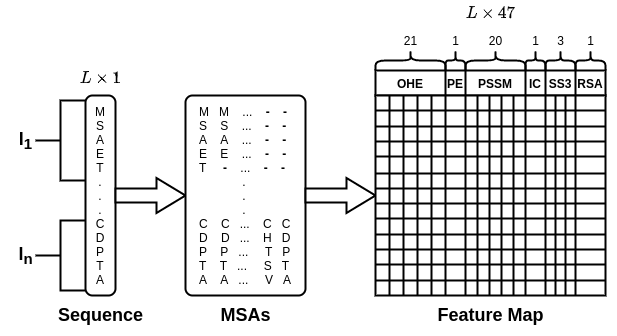
\includegraphics[scale=0.6]{feature_map}
    \caption{\centering Process used for feature map generation. The MSAs of the individual chains of a protein are generated using DeepMSA, which are used to generate the features of the protein chains. These features are concatenated to form the feature map}
    \label{fig:feature_map}
\end{figure}

\subsubsection{MSA Generation}
\quad Collections of multiple homologous sequences (called Multiple Sequence Alignments or MSAs) can provide critical information for modelling the structure and function of unknown proteins. DeepMSA \cite{zhang2020deepmsa} is an open-source method for sensitive MSA construction, which has homologous sequences and alignments created from multiple sources of databases through complementary hidden Markov model algorithms.

The search is done in 2 stages. In stage 1, the query sequence is searched against the UniClust30 \cite{mirdita2017uniclust} database using HHBlits from HH-suite\cite{remmert2012hhblits} (v2.0.16). If the number of effective sequences is $<$ 128, Stage 2 is performed where the query sequence is searched against the Uniref50 \cite{suzek2015uniref} database using JackHMMER from HMMER \cite{johnson2010hidden} (v3.1b2). Full-length sequences are extracted from the JackHMMER raw hits and converted into a custom HHBlits format database. HHBlits is applied to jump-start the search from Stage 1 sequence MSA against this custom database.

\subsubsection{One-Hot Encoding and Positional Embeddings}
\quad There are 21 amino acids in the vocabulary, 20 standard (labelled in alphabetical order from 1 to 20), and X (labelled 0, representing non-standard amino acids). The one-hot encoding (OHE) of an amino acid will be a vector of zeroes of length 21, where the position of the amino acid in the vocabulary is marked with a one. OHE is used to help the model differentiate between the different types of amino acids. Positional Embeddings (PE) carry information about the absolute position of the amino acids in the sequence. A simple method of embedding is used where the position of the $j^{th}$ amino acid is represented by ${PE}_{j} = \frac{j}{l_i}$, where $l_i$ is the length of the $i^{th}$ chain of the protein.

\newpage
\subsubsection{Position Specific Scoring Matrix and Information Content}
\quad Position Specific Scoring Matrix (PSSM) is a commonly used representation of patterns in biological sequences. PSSMs are derived from MSAs using Easel \cite{potter2018hmmer} and Heinikoff position-based weights so that similar sequences collectively contributed less to PSSM probabilities than diverse sequences. The information content (IC) of a PSSM gives an idea about how different the PSSM is from a uniform distribution. IC is also derived using Easel.

\subsubsection{Secondary Structure and Solvent Accessibility}
\quad The secondary structure is defined by the pattern of hydrogen bonds formed between the amino hydrogen and carboxyl oxygen atoms in the peptide backbone. It gives an idea of the three-dimensional structure of the protein. The secondary structural elements are alpha helices, beta sheets and turns. PSIPRED (v4.0) \cite{jones1999protein} is used to predict the probability of each state of the 3-state secondary structure (SS3) for every amino acid in the sequence. The solvent-accessible surface area is the surface area of a biomolecule that is accessible to a solvent. SOLVPRED from MetaPSICOV 2.0\cite{jones2015metapsicov} is used to predict the relative solvent accessibility (RSA) of every amino acid in the sequence. RSA can be calculated as \\ ${RSA} = {ASA} / {MaxASA}$, where ASA is the solvent-accessible surface area, and MaxASA is the maximum possible solvent accessible surface area for the amino acid residue.

% \subsubsection{SPOT-1D Features}
% \quad As a means to provide better features, SPOT-1D \cite{hanson2019improving} was used to generate the following features: solvent accessibility, half-sphere exposure, contact number, 3-state secondary structure, 8-state secondary structure, and phi, psi, theta and tau torsion angles.

% The first step in the prediction pipeline was to get the ASCII PSSM file in PSI-BLAST format. Then, hhmake was used to generate the HHM file from the MSA. SPIDER3, DCA and CCMPRED predictions were made and stored.

% The second step was to predict the contact map using SPOT-Contact, which used the previous steps predictions.

% Finally, SPOT-1D was used to make the final predictions using all the previous files as input.
% (Need to write in more detail)

\subsection{Model}
\subsubsection{Architecture}
\quad A Convolutional Neural Network (CNN) is a Deep Learning algorithm that can take an image as input, assign importance (learnable weights and biases) to various aspects/objects in the image, and differentiate one from the other. When multiple CNN layers are stacked on top of each other, Deep Neural Networks (DNNs) are formed. DNNs are difficult to train because of the vanishing gradient problem where the gradients become so small that the network's weights do not change, preventing further training. With the introduction of skip connections (shortcuts to jump over some layers) in CNNs, the vanishing gradient problem is avoided. CNNs with skip connections are known as Residual Neural Networks or ResNets\cite{he2016deep}. ResNets use representation learning to extract the most important features for classification. They can also model long-range interactions very well and hence have been very successful in the field of Computational Natural Sciences \cite{senior2020improved}.  The architecture of the deep Residual Neural Network used here is shown in Figure \ref{fig:architecture}.

Each sample protein in the dataset consists of one or more protein sequences. Let the length of the sequences be $l_1, ..., l_n$. Features are generated for each sequence in the protein (ordered by chain ID in PDB), leading to multiple vectors of shape $[l_i, 47]$ for the $i^{th}$ sequence. These generated features are combined through simple concatenation, giving a final feature vector of shape $[L, 47]$ as input to the model, where $L = l_1 + ... + l_n$.

\begin{figure}
    \centering
    \noindent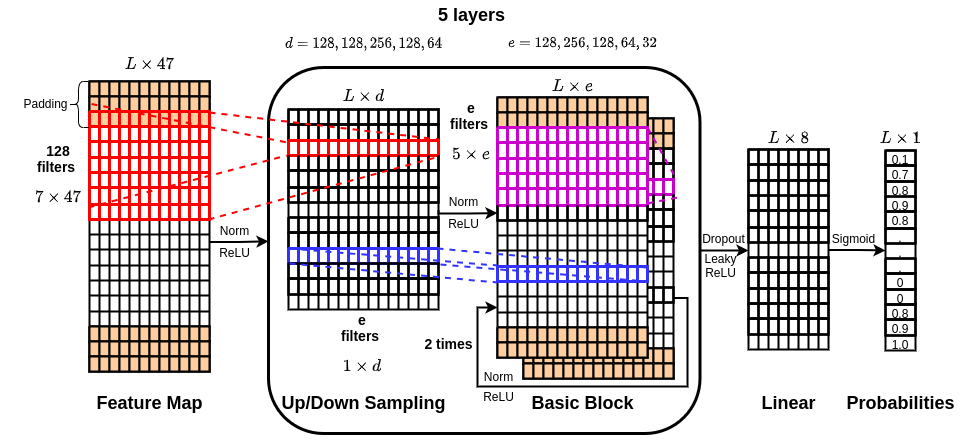
\includegraphics[scale=0.5]{architecture}
    \caption{\centering Architecture of the deep learning model, BiRDS}
    \label{fig:architecture}
\end{figure}

The feature vector is passed through the first level, consisting of a 1D convolutional layer with 128 filters, each filter size being 7, a batch normalisation layer and the ReLU (Rectified Linear Unit) activation function. The input is padded with zeroes to ensure that the length of the output vector remains the same. The filters of the convolution layer stride across the length of the protein, considering the features of the three amino acids before, the three amino acids after and the current amino acid (totalling 7). This stride along the input allows for the extraction of the required information of the current amino acid based on the features of nearby amino acids.

The following few levels consist of 2 blocks called BasicBlocks. A BasicBlock consists of a 1D convolutional layer, a batch normalisation layer, a ReLU activation function, a second 1D convolutional layer, a second batch normalisation layer, and a final ReLU activation. The skip connection is made after the final ReLU activation, where the initial input to the BasicBlock is added to the output of the final ReLU activation. Usually, the input and output size of the first BasicBlock do not match, and hence there is an up/down-sampling layer that ensures that the input has the same shape as that of the output. The output from the previous level passes through the first BasicBlock, which has an up/down-sampling layer and then goes through the second BasicBlock. In the proposed architecture, the number of filters used at each level goes from $128 \to 256 \to 128 \to 64 \to 32$, with the filter size being 5 for every convolution.

The last two levels contain a simple, linear, fully connected artificial neural network. The last but one level has a LeakyReLU activation function along with a dropout as well. The last level has a Sigmoid function to ensure that the model's output is between $[0, 1]$. The final output of the model is a vector of size $L$ (length of the protein), denoting the probabilities of a residue being a part of the binding site.

\subsubsection{Loss Function}
\quad For model training, the loss function is a weighted binary cross-entropy and is given by
$L(\hat{y}, y) = -(\alpha\hat{y}\log(y) + (1-\hat{y})\log(1-y))$, where $\hat{y}$ is the vector of true labels of whether an amino acid belongs to the binding site or not, $y$ is the model output of probabilities of a residue belonging to a binding site, $\alpha$ is the weight that is assigned to the rare class.

\newpage
The main problem in this classification task is the substantial imbalance in the two classes of binding and non-binding residues. As shown in Table \ref{tab:dataset_summary}, the percentage of binding residues is only around 6\%. Hence, $\alpha$ is used to penalise the model more heavily if it incorrectly predicts binding residues. $\alpha$ is calculated on the fly for every batch of inputs as $\alpha = \frac{n_{nbr}}{n_{br}}$, where $n_{nbr}$ is the total number of non-binding residues in the batch and $n_{br}$ is the total number of binding residues in the batch.

\subsection{Evaluation Metrics}
\subsubsection{Confusion Matrix}
A confusion matrix is a table that allows for the visualisation of the performance of a supervised learning algorithm. The following terminologies can be defined in the binary classification of a residue as a binding residue (BR) or non-binding residue (NBR).
\begin{itemize}
    \item True Positive (TP): Number of BRs predicted correctly as BRs.
    \item True Negative (TN): Number of NBRs predicted correctly as NBRs.
    \item False Positive (FP): Number of NBRs predicted incorrectly as BRs.
    \item False Negative (FN): Number of BRs predicted incorrectly as NBRs.
\end{itemize}

\noindent The following metrics can be derived from the confusion matrix

Accuracy: ${ACC} = \frac{TP + TN}{TP + TN + FP + FN}$

Precision: ${PPV} = \frac{TP}{TP + FP}$

Recall: ${TPR} = \frac{TP}{TP + FN}$

F1 score: ${F_1} = \frac{2TP}{2TP + FP + FN}$

Matthews Correlation Coefficient: ${MCC} = \frac{TP \times TN - FP \times FN}{\sqrt{(TP + FP)(TP + FN)(TN + FP)(TN + FN)}}$

\subsubsection{MCC}
\quad The Matthew's Correlation varies from $[-1, +1]$, with $+1$ representing a perfect prediction, 0 representing no better than a random prediction and -1 representing total disagreement between the prediction and the observation.

\subsubsection{DCC}
DCC is the distance between the centre of the predicted binding pocket and the centre of the actual binding pocket. It is commonly used for evaluating 3D-structure based models. The success rate of DCC is defined as the fraction of predictions below a given threshold. Predicted pockets with DCC below 4{\AA} are considered to be correctly located.

\subsection{Implementation}
\quad The model is implemented using PyTorch Lightning \cite{falcon2019pytorch}, which is a wrapper on the popular open-source deep-learning library, PyTorch \cite{paszke2019pytorch}. The model is trained in batches using an Adam Optimizer with the ReduceLROnPlateau scheduler, maximising the MCC on the validation set. A learning rate warm-up is used, where the learning rate is gradually increased to the actual learning rate during the first epoch. The implementation can be found at \href{https://github.com/devalab/BiRDS}{https://github.com/devalab/BiRDS}.

\section{Results and Discussion}
\quad The sc-PDB\cite{desaphy2015sc} dataset was split into ten folds, and ten models with the same architecture were trained. One fold formed the validation set, and the remaining folds
formed the training set for each of the models. The validation results are provided in Table \ref{tab:results}, along with the confusion matrix in Figure \ref{fig:valid_cm}

\begin{table}
    \centering
    \begin{tabular}{| P{2cm} | P{2cm} | P{2cm} | P{2cm} | P{2cm} | P{2cm} |}
        \hline
        Dataset & ACC(\%) & PPV(\%) & TPR(\%) & F1(\%) & MCC(\%) \\
        \hline
        Fold 1  & 92.58   & 48.64   & 70.65   & 57.62  & 54.83   \\
        Fold 2  & 92.18   & 46.80   & 67.29   & 55.20  & 52.08   \\
        Fold 3  & 92.94   & 44.85   & 69.37   & 54.48  & 52.27   \\
        Fold 4  & 91.28   & 39.62   & 65.73   & 49.44  & 46.72   \\
        Fold 5  & 91.74   & 46.33   & 73.11   & 56.72  & 54.07   \\
        Fold 6  & 92.19   & 47.16   & 69.70   & 56.25  & 53.34   \\
        Fold 7  & 91.90   & 45.45   & 69.55   & 54.98  & 52.13   \\
        Fold 8  & 92.52   & 47.58   & 68.16   & 56.04  & 53.10   \\
        Fold 9  & 92.06   & 41.86   & 69.69   & 52.31  & 50.14   \\
        Fold 10 & 92.08   & 44.54   & 68.88   & 54.10  & 51.41   \\
        Test    & 94.05   & 50.46   & 67.45   & 57.73  & 55.27   \\
        \hline
    \end{tabular}
    \caption{\label{tab:results} Validation results of all 10 trained models and test results}
\end{table}

\begin{figure}
    \centering
    \noindent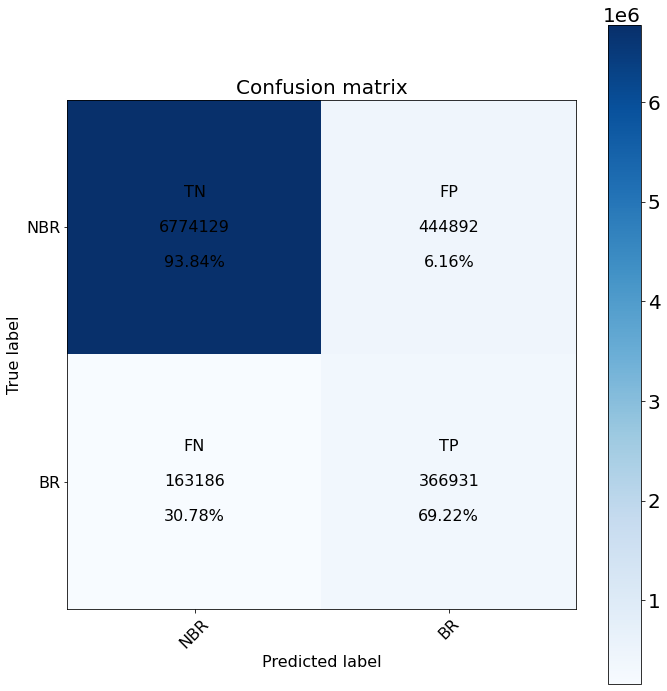
\includegraphics[scale=0.4]{valid_cm.png}
    \caption{\centering Sum of confusion matrices of the 10 models on their corresponding validation set}
    \label{fig:valid_cm}
\end{figure}

\newpage
For testing, the ten trained models are run on the test set. An amino acid belongs to the binding site for the consensus algorithm if five or more models predict the same. The test results are also provided in Table \ref{tab:results}, along with the confusion matrix in Figure \ref{fig:test_cm}

\begin{figure}
    \centering
    \noindent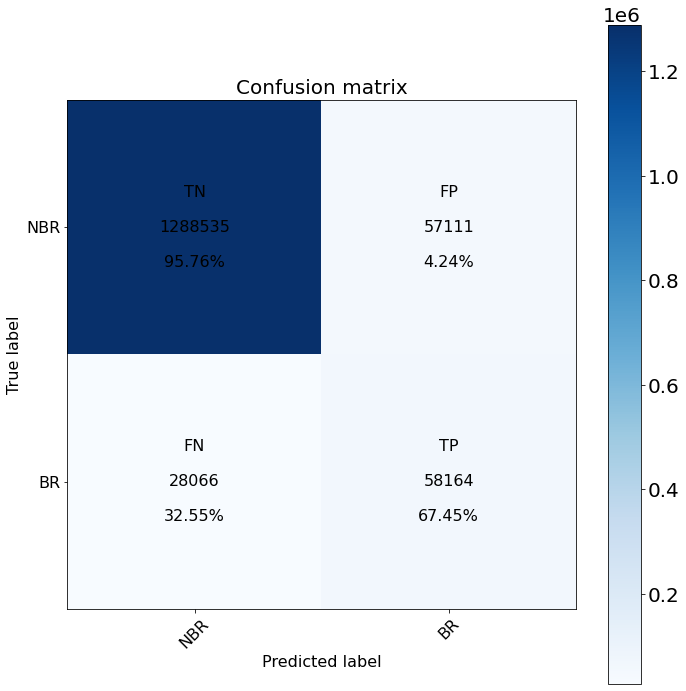
\includegraphics[scale=0.4]{test_cm.png}
    \caption{\centering Confusion matrix on the test set after averaging the predictions of the 10 models}
    \label{fig:test_cm}
\end{figure}

The model predictions were mapped back to the available 3D structures of proteins for the calculation of DCC. Figure \ref{fig:valid_dcc} denotes the cross-validation results. The deep learning model is the same across all ten splits of training and validation datasets. The success rate of the models varies based on the fold that is used for validation. It ranges from 33\% to 49\% success rate when the DCC threshold is less than 4\AA. Figure \ref{fig:test_dcc} denotes the test result. The predictions have a 40\% success rate when the DCC threshold is less than 4\AA, meaning that for 40\% of the test data, the model has predicted the binding site such that the centre of the predicted binding site is within 4\AA \ of the centre of the true binding site. As the threshold of DCC increases, the success rate also naturally increases. One should note that even if the model predicts the whole binding site correctly and misses out on a couple of residues or predicts more residues, the centre of the predicted binding site will change significantly.

\begin{figure}
    \centering
    \noindent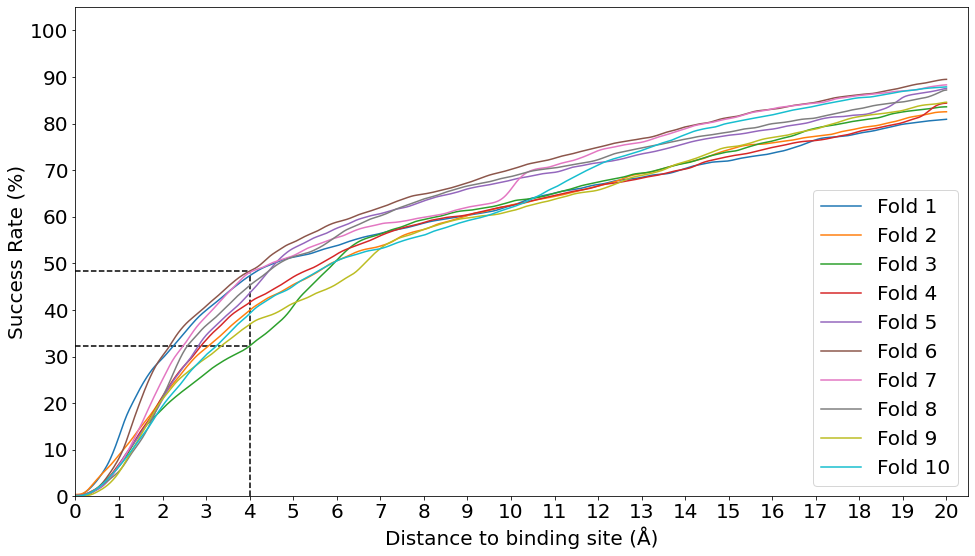
\includegraphics[scale=0.45]{valid_dcc.png}
    \caption{\centering Success rate plot for various DCC thresholds of the 10 models on their corresponding validation set}
    \label{fig:valid_dcc}
\end{figure}

\begin{figure}
    \centering
    \noindent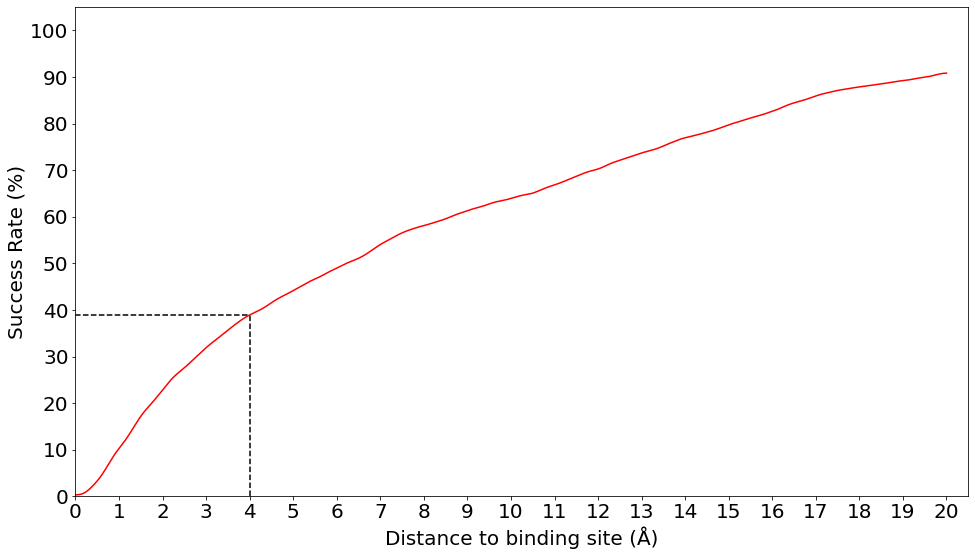
\includegraphics[scale=0.45]{test_dcc.png}
    \caption{\centering Success rate plot for various DCC thresholds on the test set after averaging the predictions of the 10 models}
    \label{fig:test_dcc}
\end{figure}

On their test set, DeepSite, a 3D structure-based deep learning model \cite{jimenez2017deepsite} achieved around 40\% success rate. Given that our model uses only the amino acid sequence information, its performance is commendable. Even though the test sets are not the same, it still gives an idea of how well the current model performs.

All the currently available methods for predicting the binding site of a protein, based on sequence, predict the site only for a specific set of ligands, while our model predicts the most ligandable binding site irrespective of the ligand. Hence, there is no available method of comparison with our model for the sequence-based prediction of binding residues on the sc-PDB\cite{desaphy2015sc} dataset.

As a simple way to test the effectiveness of our model against DeepCSeqSite's model, we followed two approaches:
\begin{enumerate}
    \item Run the trained DeepCSeqSite model on our test set
    \item Reimplement DeepCSeqSite model architecture, train on our dataset, and then test
\end{enumerate}

Both approaches failed to provide good results, with approach one providing an MCC score of 0.05 and approach two providing an MCC score of 0.1. The failure in approach one could be due to the difference in the method for generating the MSAs.

A variety of deep learning models such as Complementary GANs, stacked BiLSTMs, and TAPE protein embeddings were used for training as a means to improve the predictions. Features, such as backbone angles, secondary structure, solvent accessibility and contact number, generated using SPOT-1D \cite{hanson2018accurate} were also tried as features. None of them provided any significant improvement over vanilla ResNets and simple features. Instead, they added unnecessary, additional computational costs.

% \subsection{Experiments}

% TAPE Embeddings (Both embeddings) and as a downstream task

% Complementary GAN to try and solve the imbalance

% Using SPOT-1D features

% BiLSTMs, UNet, Transformers

% Window of features using predicted contact maps

% Training on chains separately

\quad Some case studies were undertaken to show that the model performs as expected, but the metrics do not rate it well due to limitations of the dataset. The aggregated predictions of the models on the test set were mapped back to the three-dimensional structure of the protein-ligand complex to see how good the predictions are. The 3-D structures were generated using 3Dmol.js\cite{rego20153dmol}. In the following examples, the colour red indicates an incorrect prediction of the amino acid as a binding residue. Blue indicates an amino acid that is a binding residue but was not predicted as binding by the model. Green indicates an amino acid that was correctly predicted as binding.

In Figure \ref{fig:5ymx}, it looks like the model is mispredicting everything for 5YMX\cite{galicia2019mgla}, but it is predicting another binding site of the protein. The sc-PDB\cite{desaphy2015sc} dataset was generated through a series of filters, and the residues surrounding the most buried ligand was selected to be the most ligandable binding site. This selection, unfortunately, is a flaw of the dataset and the method used for predictions. There is no right way to cover cases like these where the model needs to be penalised less when it predicts a binding site that is not the most ligandable binding site. Hence, the evaluation metrics used will generally give an abysmal score for such cases.
\begin{figure}
    \centering
    \noindent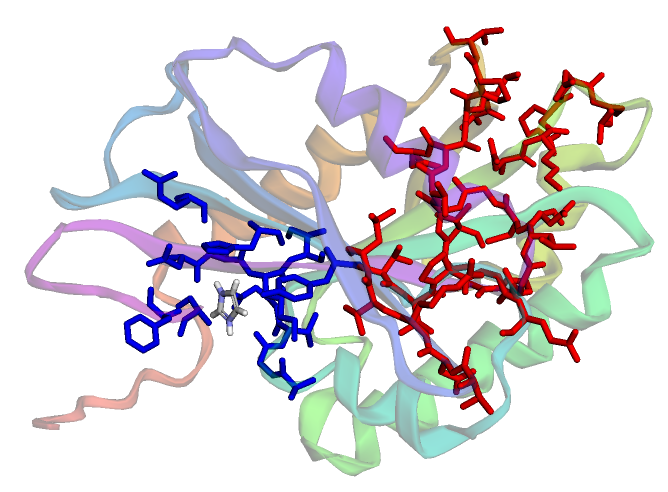
\includegraphics[scale=0.4]{5ymx.png}
    \caption{\centering 5YMX - The model seems to be mispredicting the actual binding site (in blue), but is in fact, predicting another binding site of the protein (in red)}
    \label{fig:5ymx}
\end{figure}

Figure \ref{fig:6hu9} shows 6HU9\cite{maldonado2021atomic}, where the model predicts individual binding sites of two proteins with the same sequence, but it finds it difficult to predict the binding site created due to the interaction between the two proteins. This may be due to the way the features are generated. It is not easy to generate features of the protein since the MSAs are generated for individual chains of a protein, not providing any information about the interaction between the chains. Due to the fewer samples containing a binding site between the interaction of protein chains, the model fails to learn the same.
\begin{figure}
    \centering
    \noindent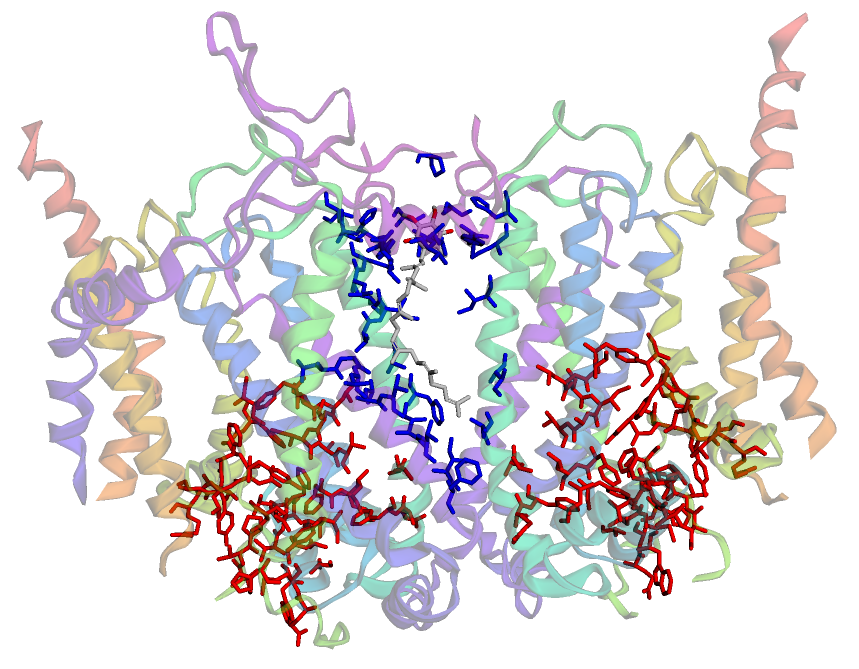
\includegraphics[scale=0.35]{6hu9.png}
    \caption{\centering 6HU9 - The model is able to predict the individual binding site of the protein  (in red), but not the interaction binding site (in blue)}
    \label{fig:6hu9}
\end{figure}

Figure \ref{fig:6pf6} shows 6PF6\cite{czyzyk2019structure}, where the model predicts the binding site with good accuracy. It can be seen that it predicts most of the residues around the binding site and also a couple more just outside the binding site. Since the two chains of the protein have the same sequence, the model predicts identical binding residues for both chains. sc-PDB selects only one binding site as the most active binding site, and therefore, only that site is used for calculating the metrics. The metrics do not do justice to these types of predictions and score the model very poorly, even though it is doing very well.
\begin{figure}
    \centering
    \noindent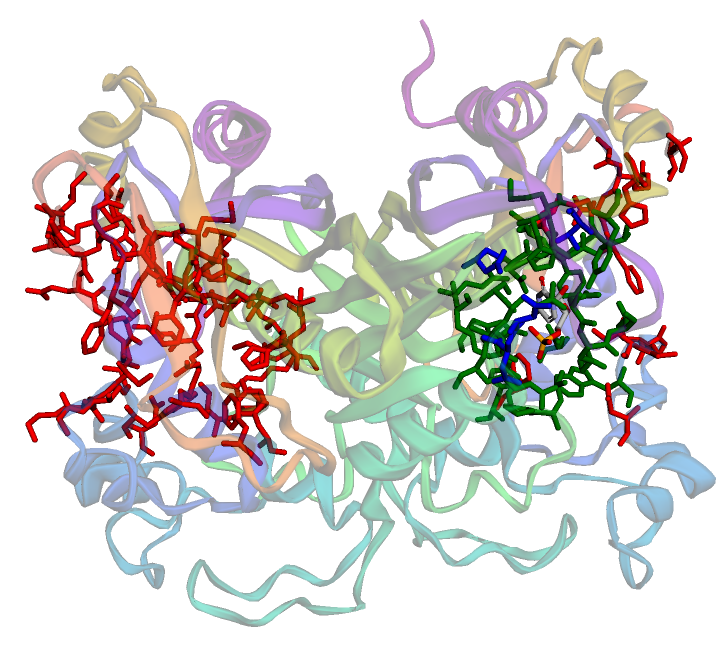
\includegraphics[scale=0.4]{6pf6.png}
    \caption{\centering 6PF6 - The model predicts the binding site correctly, but due to the presence of the same chains in the protein, it predicts both the binding sites (in green and red)}
    \label{fig:6pf6}
\end{figure}

\newpage
\section{Conclusion}
In this study, a ResNet was used to predict the most active binding site of a protein. The sc-PDB\cite{desaphy2015sc} dataset contained data of the most ligandable binding site of a protein. MSAs were generated for all protein chains in the dataset using DeepMSA, and features such as Position-Specific Scoring Matrix, Secondary Structure and Solvent Accessibility were calculated. A new test set, SC6K, considering proteins in the last three years, was made using the same filters used to create the sc-PDB dataset. The individual features of the protein chains were concatenated, and the ResNet was trained using 10-fold cross-validation. The ResNet can predict the binding site of a protein fairly accurately using only the sequence information. In drug design, it becomes crucial to determine the pocket where the drug molecule binds with the protein. BiRDS (our method) can be used for early and quick determination of the binding site before the availability of the protein structure.

\begin{acknowledgement}
    The authors thank Yashaswi Pathak for being a fruitful part of the project discussions and Rishal Aggarwal and Akash Gupta for reviewing the manuscript. We acknowledge IHub-Data, IIIT Hyderabad for financial support and access to high-performance clusters for running computations.
\end{acknowledgement}

\bibliography{achemso-demo}

\end{document}
